% === NỘI DUNG: TỔNG QUAN HỆ THỐNG DRONE CỨU HỘ ===

\subsection{Tổng quan về UAV và ứng dụng trong cứu hộ cứu nạn}

Thiết bị bay không người lái (UAV -- Unmanned Aerial Vehicle) là một loại phương tiện hàng không được điều khiển từ xa hoặc hoạt động theo chương trình lập sẵn, không có phi công trên khoang. Trong những thập kỷ gần đây, UAV dân sự đã trải qua sự phát triển bùng nổ, từ các mô hình đơn giản dùng cho chụp ảnh trên không đến các hệ thống phức tạp tích hợp cảm biến đa phương thức và trí tuệ nhân tạo.

Theo phân loại hình thức cấu trúc khung thân, UAV dân sự phổ biến nhất hiện nay bao gồm:
\begin{itemize}
    \item \textbf{Quadcopter (4 cánh quạt)}: Cấu trúc đơn giản, dễ điều khiển, chi phí thấp, phù hợp cho các nhiệm vụ giám sát và cứu hộ tầm gần. Tiêu biểu là DJI Phantom, DJI Mavic và Parrot Anafi.
    \item \textbf{Hexacopter/Octocopter}: Cung cấp khả năng dự phòng động cơ và tải trọng lớn hơn, thường được dùng cho nhiệm vụ chuyên nghiệp như chụp ảnh điện ảnh hoặc giao hàng.
    \item \textbf{Fixed-wing UAV}: Hiệu quả năng lượng cao, tầm hoạt động xa, nhưng đòi hỏi không gian cất hạ cánh và không thể bay tại chỗ (hover).
    \item \textbf{Hybrid VTOL}: Kết hợp ưu điểm của cả hai loại trên, có khả năng cất hạ cánh thẳng đứng và chuyển đổi sang chế độ cánh cố định.
\end{itemize}

Trong lĩnh vực tìm kiếm cứu nạn (SAR -- Search and Rescue), Quadcopter được ưu tiên sử dụng nhờ khả năng hover ổn định tại chỗ, cơ động cao trong không gian hẹp, triển khai nhanh và chi phí đầu tư thấp. Các nghiên cứu gần đây \cite{Goodrich2008} chỉ ra rằng UAV có thể giảm thời gian tìm kiếm nạn nhân trong các vùng địa hình phức tạp xuống còn 15--20\% so với phương pháp truyền thống.

\begin{figure}[H]
    \centering
    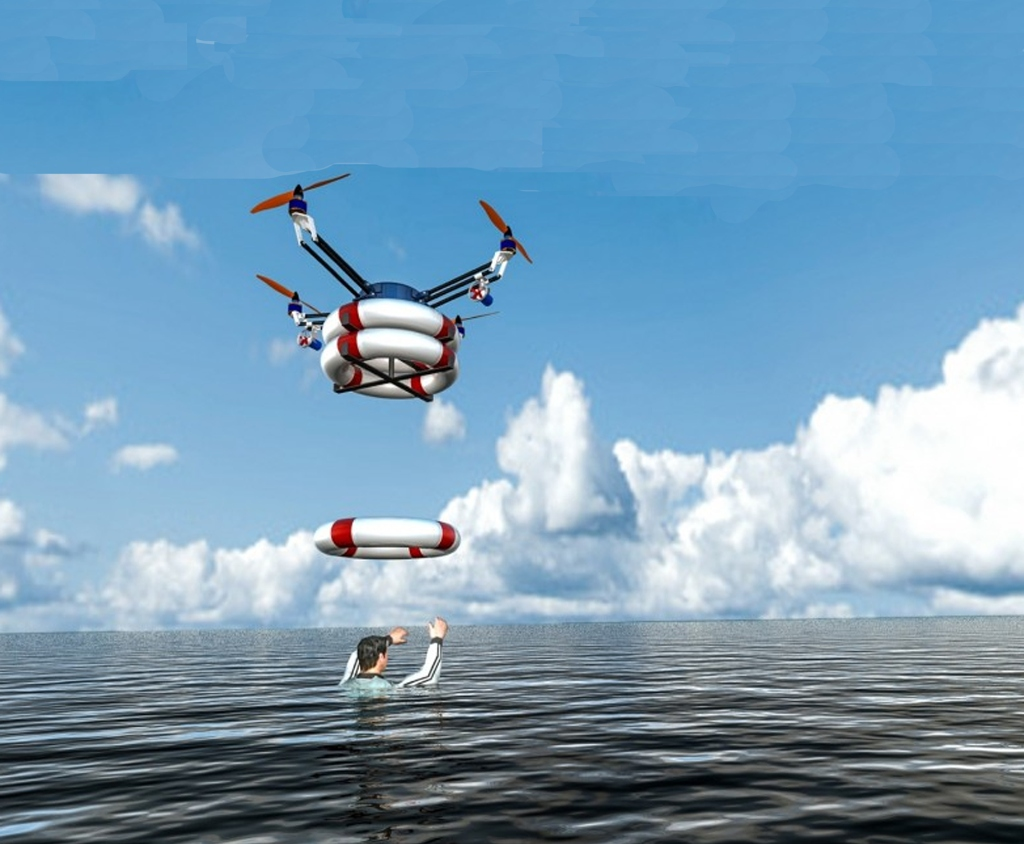
\includegraphics[width=0.8\textwidth]{Images/cuu_ho_sar.jpg}
    \caption[Hình ảnh minh họa hoạt động tìm kiếm cứu nạn bằng Drone]{\bfseries\fontsize{12pt}{0pt}\selectfont Hình ảnh minh họa hoạt động tìm kiếm cứu nạn bằng Drone}
    \label{fig:cuu_ho_sar}
\end{figure}


\subsection{Tình hình nghiên cứu trong và ngoài nước}

\subsubsection{Nghiên cứu quốc tế}

Trên thế giới, các nghiên cứu về UAV cứu hộ thông minh đã đạt được những kết quả đáng kể:

\begin{itemize}
    \item Hệ thống SHERPA (2013--2017) do Liên minh Châu Âu tài trợ đã phát triển đội UAV và UGV (robot mặt đất) phối hợp tìm kiếm nạn nhân trong các vụ lở tuyết, tích hợp camera nhiệt và nhận diện hình người \cite{DellAmore2014}.
    \item DJI và Parrot đã thương mại hóa các giải pháp UAV tích hợp camera nhiệt FLIR cho nhiệm vụ SAR ban đêm, được sử dụng rộng rãi bởi các đội cứu hộ tại Mỹ, Anh và Đức.
    \item Nghiên cứu của Bejiga et al. (2017) tại Na Uy đề xuất sử dụng mạng nơ-ron tích chập CNN để phát hiện người trong ảnh hồng ngoại từ UAV, đạt độ chính xác trên 85\% trong điều kiện tuyết trắng.
    \item Các nền tảng tự động bay phổ biến như ArduPilot (APM/Pixhawk) và Betaflight (cho FPV racing) đã cung cấp firmware mã nguồn mở cho cộng đồng nghiên cứu. Đề tài này lựa chọn phát triển firmware riêng trên STM32 để nắm sâu nguyên lý điều khiển.
\end{itemize}

\subsubsection{Nghiên cứu trong nước}

Tại Việt Nam, nghiên cứu về UAV cứu hộ đang trong giai đoạn phát triển:

\begin{itemize}
    \item Một số trường đại học như Đại học Bách Khoa Hà Nội, Học viện Kỹ thuật Quân sự đã nghiên cứu phát triển hệ thống điều khiển UAV dựa trên các nền tảng mã nguồn mở như ArduPilot và PX4.
    \item Tuy nhiên, phần lớn các nghiên cứu trong nước chủ yếu tập trung vào việc ứng dụng phần cứng thương mại sẵn có (Pixhawk, Naza-M) mà chưa đi sâu vào việc tự thiết kế Flight Controller từ đầu trên nền tảng vi điều khiển ARM nhúng.
    \item Hướng tích hợp AI -- cụ thể là YOLOv8 -- trực tiếp vào quy trình giám sát cứu hộ từ UAV vẫn là hướng nghiên cứu mới tại các trường kỹ thuật trong nước.
\end{itemize}

\subsection{Các công nghệ nền tảng được sử dụng trong đề tài}

\subsubsection{Vi điều khiển STM32F103C8T6 (ARM Cortex-M3)}

STM32F103C8T6 là vi điều khiển 32-bit thuộc dòng STM32F1 của STMicroelectronics, xây dựng trên lõi ARM Cortex-M3. Với tần số hoạt động tối đa 72\,MHz, bộ nhớ Flash 64\,KB, SRAM 20\,KB, đây là lựa chọn phổ biến cho các ứng dụng điều khiển nhúng thời gian thực nhờ khả năng xử lý mạnh mẽ, tiết kiệm năng lượng và hỗ trợ nhiều giao tiếp ngoại vi phong phú.

\begin{figure}[H]
    \centering
    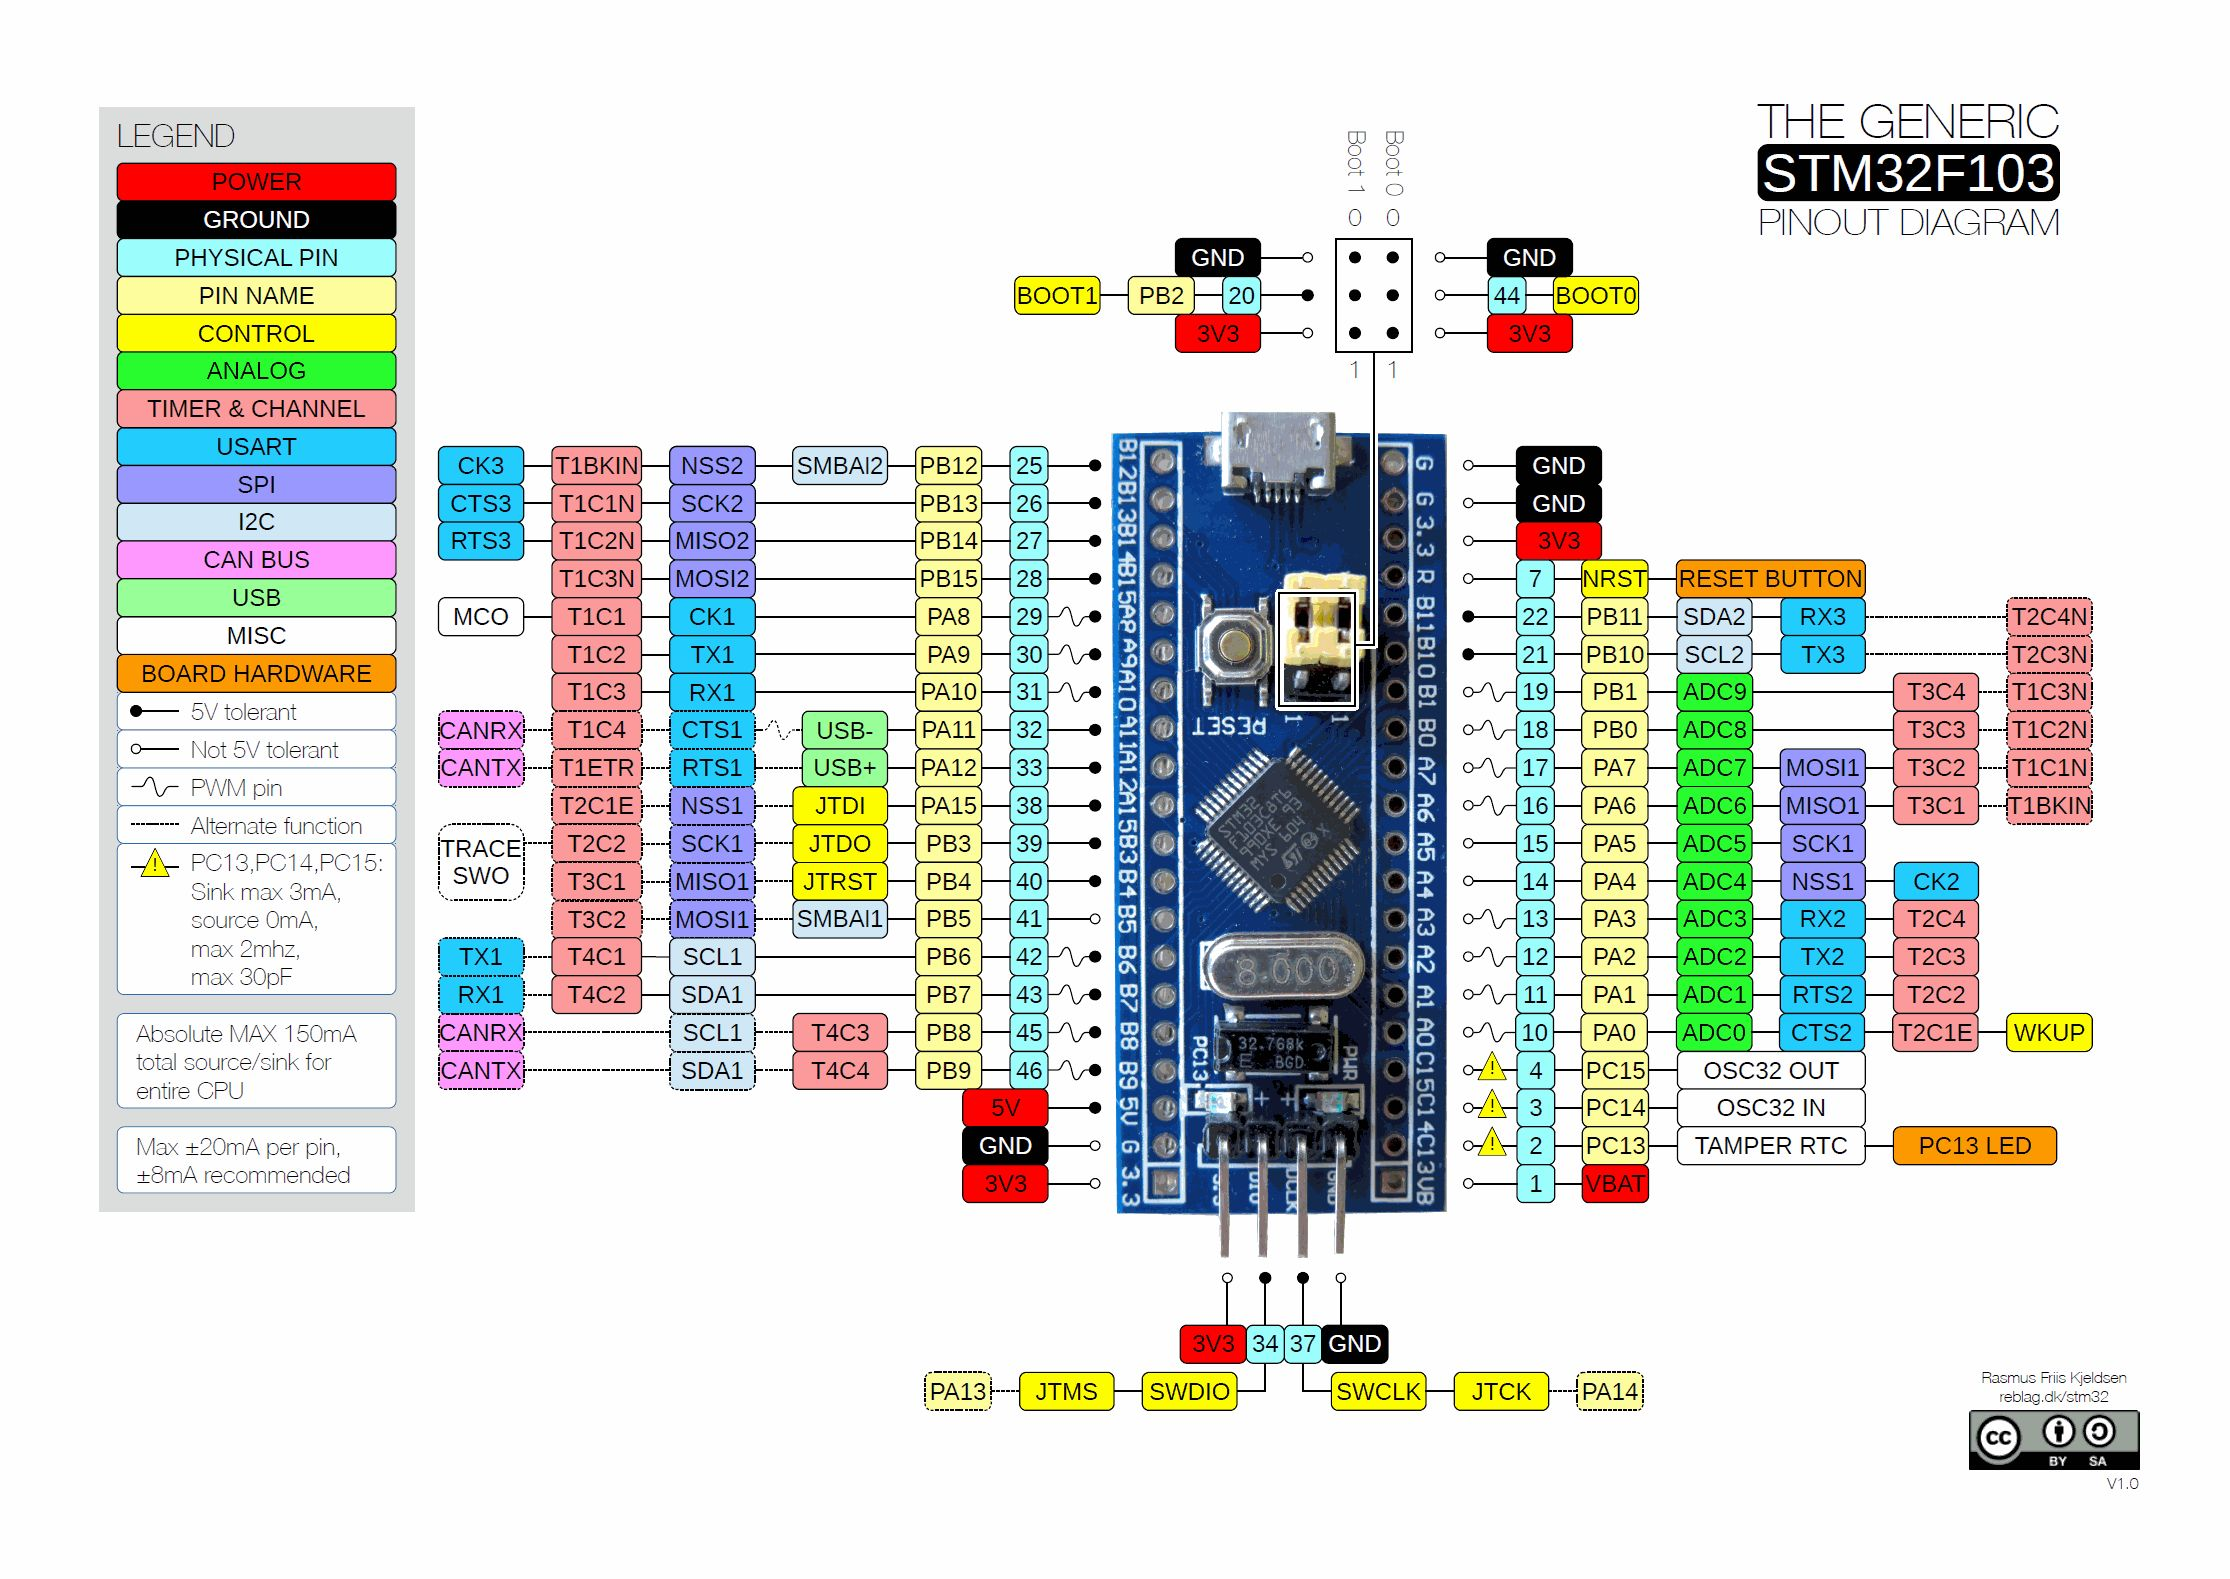
\includegraphics[width=0.6\textwidth]{Images/linhkien/stm32f103c8t6.jpg}
    \caption{Vi điều khiển STM32F103C8T6 (Dòng Blue Pill 48 chân)}
    \label{fig:stm32_ch1}
\end{figure}

\begin{table}[H]
    \centering
    \caption{Thông số kỹ thuật chính của STM32F103C8T6}
    \label{tab:stm32_specs}
    \begin{tabular}{|c|c|}
        \hline
        \textbf{Thông số} & \textbf{Giá trị} \\ \hline
        Bộ xử lý & ARM\textregistered\ Cortex\textregistered-M3 32-bit \\ \hline
        Tần số hoạt động & Lên đến 72\,MHz \\ \hline
        SRAM & 20\,KB \\ \hline
        Flash & 64\,KB \\ \hline
        Điện áp hoạt động & 2.0\,V -- 3.6\,V \\ \hline
        ADC & 2 bộ 12-bit (10 kênh đầu vào) \\ \hline
        UART & 3 bộ \\ \hline
        SPI & 2 bộ \\ \hline
        I2C & 2 bộ \\ \hline
        Số chân GPIO & Tối đa 37 chân (loại 48 chân) \\ \hline
    \end{tabular}
\end{table}

Trong đồ án này, STM32F103C8T6 được sử dụng làm bộ vi điều khiển trung tâm (Flight Controller) của toàn bộ hệ thống Drone. Mạch nhận nhiệm vụ thu thập dữ liệu góc thô từ cảm biến quán tính MPU6050 qua chuẩn giao tiếp I2C tốc độ cao, đồng thời đọc tín hiệu điều khiển từ bộ thu phát vô tuyến ELRS qua giao tiếp UART. Qua quá trình xử lý tín hiệu và tính toán thuật toán PID vòng lặp kép, chip vi điều khiển sẽ xuất xung PWM để điều khiển các động cơ không chổi than (thông qua ESC), giúp Drone giữ thăng bằng và phản hồi chính xác theo quỹ đạo điều khiển.

\subsubsection{Cảm biến quán tính IMU MPU6050}

MPU-6050 là module cảm biến quán tính 6-DoF (Degree of Freedom) của InvenSense, tích hợp đồng thời cảm biến gia tốc kế 3 trục (Accelerometer) và con quay hồi chuyển 3 trục (Gyroscope) trong cùng một chip. Giao tiếp qua giao thức I2C hoặc SPI. Chip này cũng tích hợp sẵn bộ xử lý tín hiệu số DMP (Digital Motion Processor) có thể ước lượng tư thế cơ bản, tuy nhiên trong đề tài ta sẽ đọc dữ liệu thô và tự cài đặt bộ lọc bù để nắm rõ nguyên lý.

\begin{figure}[H]
    \centering
    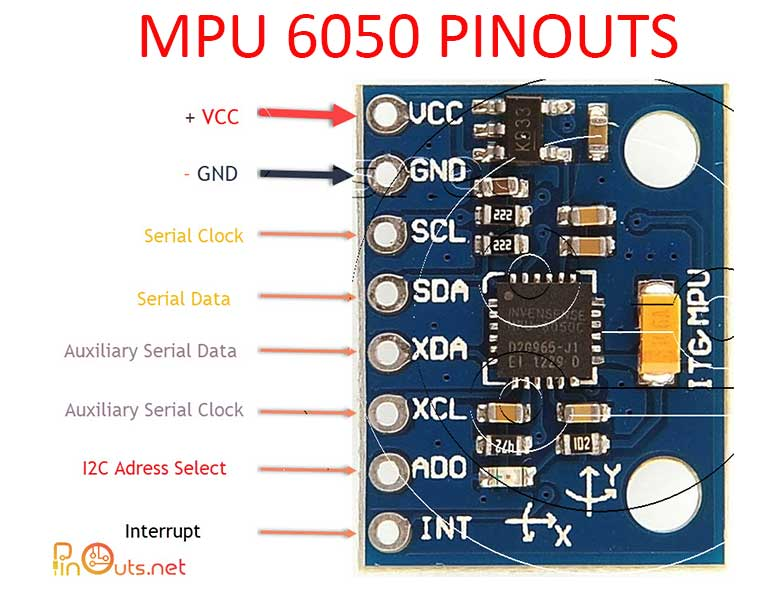
\includegraphics[width=0.45\textwidth]{Images/linhkien/mpu6050.jpg}
    \caption{Module cảm biến quán tính IMU MPU6050}
    \label{fig:mpu6050_ch1}
\end{figure}

\subsubsection{Giao thức điều khiển vô tuyến ExpressLRS (ELRS)}

Hệ thống điều khiển bay từ xa trong đồ án sử dụng giao thức truyền thông mã nguồn mở ExpressLRS (ELRS). Đây là giao thức thế hệ mới được thiết kế đặc biệt cho UAV FPV, nổi bật với:
\begin{itemize}
    \item Độ trễ cực thấp: 1--4\,ms tùy tốc độ packet.
    \item Tần số truyền gói điều khiển: lên đến 1000\,Hz ở chế độ 1000\,Hz Packet Rate.
    \item Phạm vi hoạt động lớn: tới vài km với công suất phát 250\,mW.
    \item Chuẩn giao tiếp với FC: giao thức CRSF (Crossfire Serial) trên UART.
\end{itemize}

Hệ thống điều khiển bao gồm hai thiết bị chính:

\paragraph{Tay điều khiển phát sóng (TX - RadioMaster Pocket)}

Tay cầm điều khiển (Transmitter) RadioMaster Pocket được tích hợp sẵn module phát sóng ELRS tần số 2.4\,GHz. Thiết bị này đọc vị trí góc nghiêng của các cần gạt (joystick), mã hóa thành gói tin CRSF và truyền đi với độ trễ cực thấp. Thiết bị hỗ trợ tốc độ truyền gói tin điều khiển cực cao (lên tới 500\,Hz) với công suất phát linh hoạt, mang lại độ nhạy sóng cao và cự ly điều khiển ổn định đạt hàng kilômét trong điều kiện khuất địa hình.
\begin{figure}[H]
    \centering
    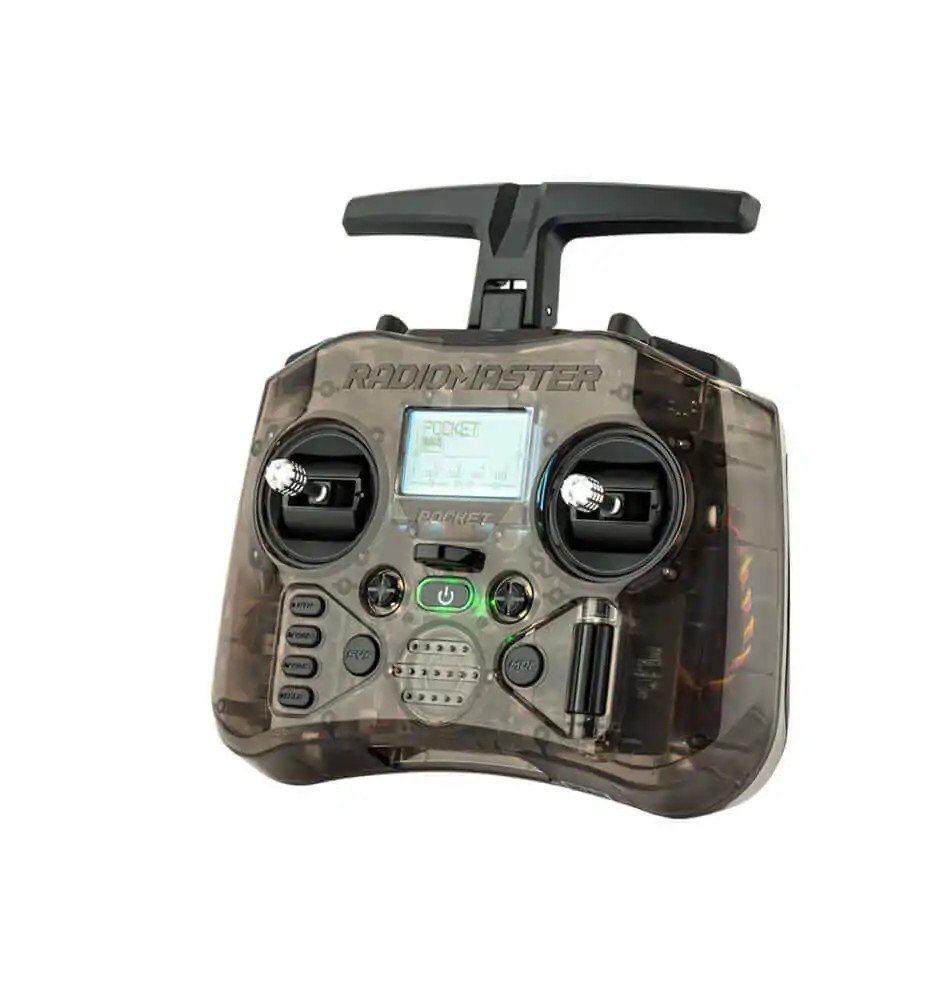
\includegraphics[width=0.45\textwidth]{Images/rm_pocket.png}
    \caption{Tay điều khiển phát sóng RadioMaster Pocket (TX)}
    \label{fig:rm_pocket_ch1}
\end{figure}

\paragraph{Module thu sóng (RX - Cyclone ELRS 2.4GHz 7CH)}

Mạch thu sóng siêu nhỏ (Receiver) được lắp đặt trực tiếp trên Drone. Module có nhiệm vụ nhận gói tin tần số cao từ tay phát và kết nối với Flight Controller thông qua giao thức truyền thông UART nối tiếp tốc độ cao sử dụng chuẩn giao thức CRSF (Crossfire) với tốc độ baud mặc định là 420.000\,bps. Dòng dữ liệu nối tiếp nguyên bản sẽ được đẩy vào vi điều khiển STM32F103C8T6 để giải mã lệnh bay, giúp giảm thiểu tối đa độ trễ.
\begin{figure}[H]
    \centering
    
\includegraphics[width=0.4\textwidth]{Images/linhkien/elrs_rx.png}
    \caption{Module thu tín hiệu vô tuyến ExpressLRS (RX)}
    \label{fig:elrs_rx_ch1}
\end{figure}

\subsubsection{Camera FPV và hệ thống truyền hình ảnh VTX/VRX}

Hệ thống truyền hình ảnh analog FPV (First-Person View) trong đồ án đóng vai trò thu thập và truyền tải video thời gian thực từ Drone về trạm mặt đất để phục vụ mô hình AI phân tích. Hệ thống bao gồm 3 thành phần chính:

\paragraph{Camera FPV (Caddx Ant Lite)}

Camera Caddx Ant Lite chuyên dụng cho thiết bị bay sở hữu cảm biến CMOS 1/3 inch, độ phân giải sắc nét 1200\,TVL và tích hợp dải động cao Global WDR giúp duy trì khả năng quan sát tốt nạn nhân trong môi trường ngược sáng mạnh. Trọng lượng camera siêu nhẹ (2\,g) và độ trễ truyền dẫn tín hiệu analog gần như bằng 0 (dưới 10\,ms) là các yếu tố then chốt cho hệ thống FPV. Camera xuất trực tiếp tín hiệu video analog chuẩn NTSC/PAL với độ nhạy sáng cao.
\begin{figure}[H]
    \centering
    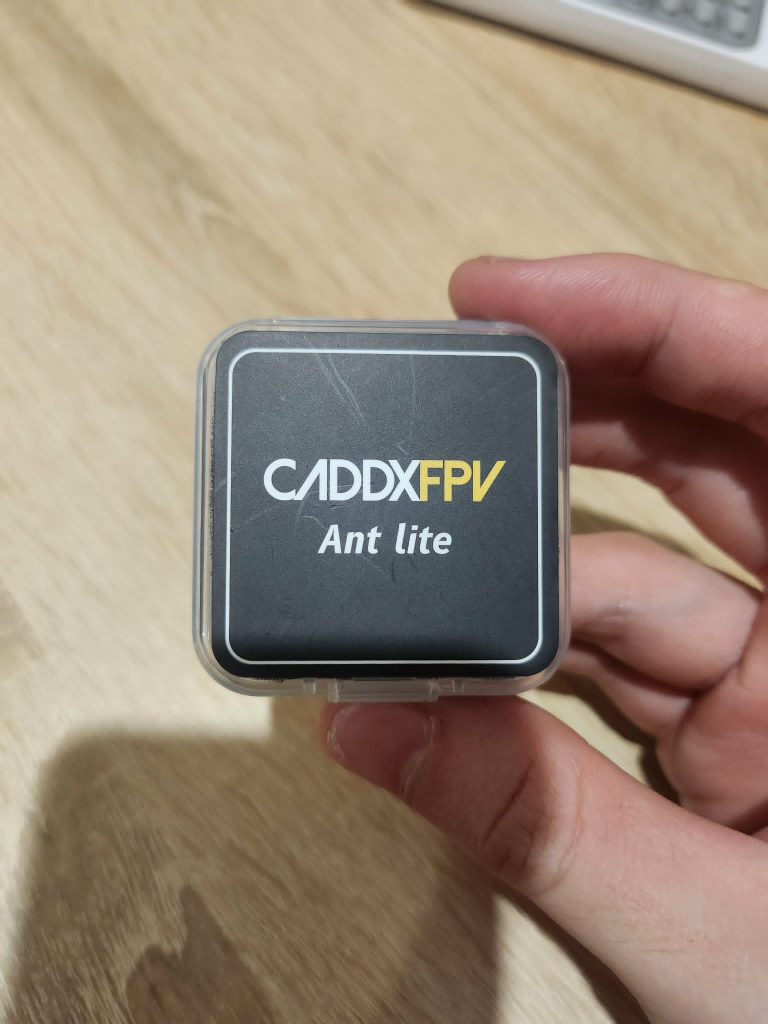
\includegraphics[width=0.35\textwidth]{Images/caddx_cam.png}
    \caption{Camera FPV Caddx Ant Lite}
    \label{fig:caddx_cam_ch1}
\end{figure}

\paragraph{Module phát video VTX (Cyclone VTX 5.8GHz)}

Cyclone VTX là module phát sóng video analog hoạt động ở băng tần 5.8\,GHz. Mạch có công suất phát tối đa lên tới 1000\,mW để truyền tín hiệu từ camera về trạm mặt đất. Thiết bị hỗ trợ phím nhấn vật lý kết hợp LED trạng thái trực quan để chuyển đổi linh hoạt giữa các dải tần số (Band A/B/E/F/R), các kênh phát (CH1-CH8) và mức công suất (25/100/200/400/1000\,mW), giúp người vận hành dễ dàng tối ưu hóa chất lượng sóng truyền hình ảnh và tránh hiện tượng nhiễu xuyên kênh.
\begin{figure}[H]
    \centering
    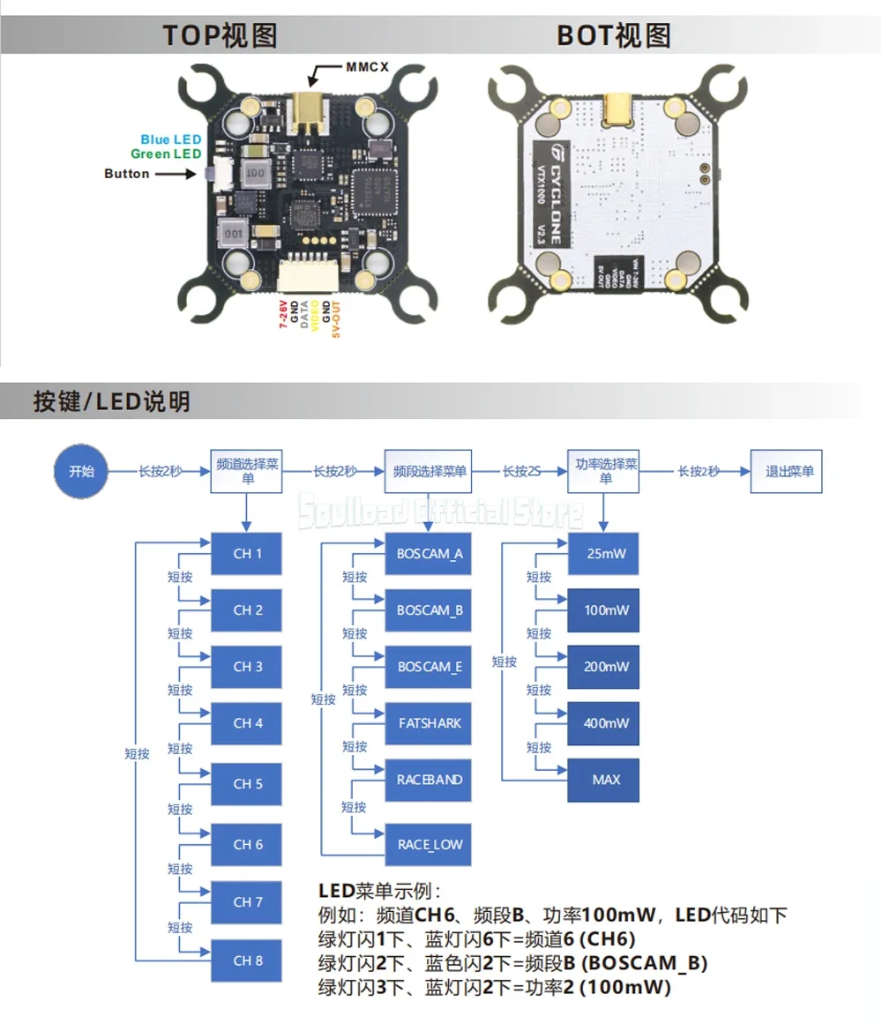
\includegraphics[width=0.4\textwidth]{Images/cyclone_vtx.png}
    \caption{Module phát hình ảnh Cyclone VTX 5.8GHz}
    \label{fig:cyclone_vtx_ch1}
\end{figure}

\paragraph{Module thu video VRX (Skydroid 5.8G OTG)}

Trạm mặt đất sử dụng bộ thu hình chuyên dụng Skydroid 5.8G OTG Receiver. Bộ thu tự động dò quét và đồng bộ hóa tần số phát sóng của VTX qua 150 kênh sóng. Video thu được được chuyển đổi sang chuẩn tín hiệu số và truyền trực tiếp vào máy tính trạm mặt đất GCS thông qua kết nối USB dạng UVC (OTG), giúp phần mềm AI Python dễ dàng đọc luồng video và thực thi nhận diện mà không cần thêm thiết bị Capture rời nào.
\begin{figure}[H]
    \centering
    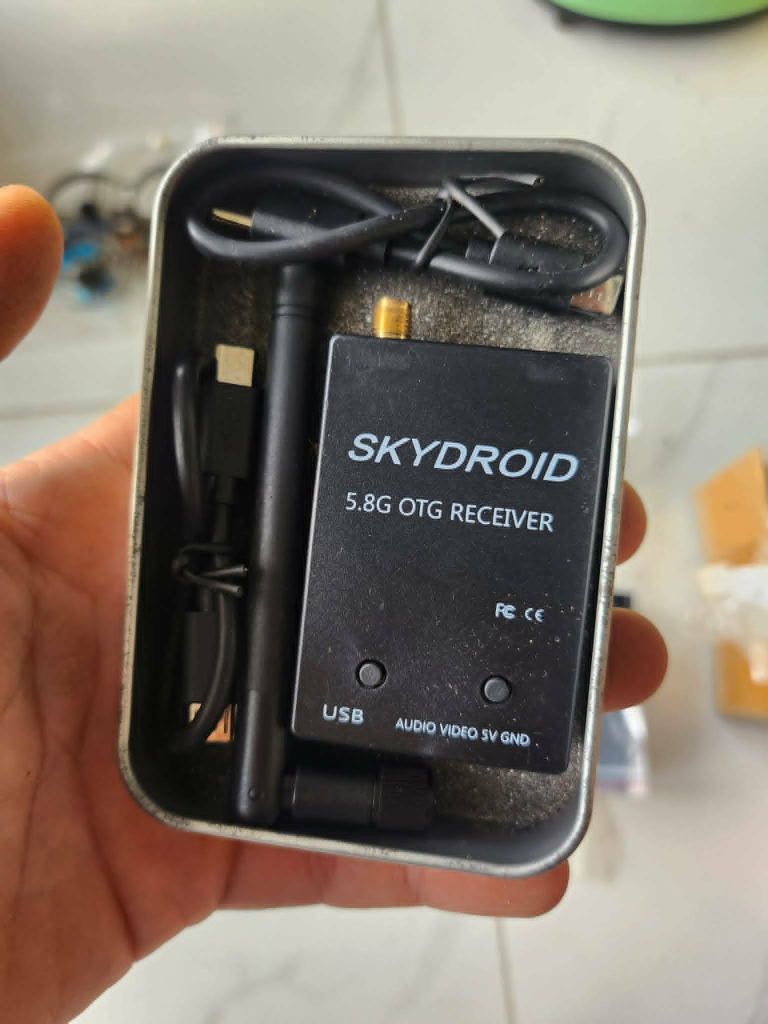
\includegraphics[width=0.4\textwidth]{Images/skydroid_vrx.png}
    \caption{Thiết bị thu và số hóa hình ảnh Skydroid 5.8G OTG VRX}
    \label{fig:skydroid_vrx_ch1}
\end{figure}

Việc sử dụng trọn bộ hệ thống analog FPV này mang lại ưu điểm vượt trội về độ trễ đầu cuối (end-to-end latency thấp hơn 40\,ms) so với các giải pháp IP Camera kỹ thuật số, hoàn toàn đáp ứng được yêu cầu cập nhật theo thời gian thực của thuật toán phát hiện nạn nhân.



\subsection{Xác định khoảng trống nghiên cứu và hướng tiếp cận của đề tài}

Qua phân tích tổng quan, có thể nhận thấy các khoảng trống nghiên cứu sau:

\subsubsection{Thiếu nghiên cứu tự thiết kế FC nhúng ARM cho UAV cứu hộ trong nước}
Phần lớn đề tài trong nước dùng FC thương mại, không đi sâu vào thiết kế phần cứng từ đầu. Đề tài này lấp đầy khoảng trống này bằng cách tự thiết kế PCB và lập trình firmware hoàn toàn trên STM32F103.

\subsubsection{Thiếu hệ thống AI đa mô hình dung hợp quyết định cho bài toán cứu hộ}
Các nghiên cứu hiện tại thường chỉ dùng một mô hình đơn lẻ (phát hiện người) mà chưa kết hợp đa mô hình đánh giá trạng thái nguy hiểm. Đề tài đề xuất thuật toán dung hợp ba mô hình YOLOv8 tính Danger Score toàn cục.

\subsubsection{Thiếu tích hợp từ đầu đến cuối}
Phần cứng Drone và hệ thống AI thường được nghiên cứu tách biệt. Đề tài này cung cấp một giải pháp tích hợp từ thiết kế cơ khí, điện tử đến phần mềm AI, tạo thành một hệ thống hoàn chỉnh.

\textbf{Hướng tiếp cận} của đề tài là kết hợp phương pháp từ dưới lên (Bottom-up): bắt đầu từ thiết kế linh kiện phần cứng cơ bản, xây dựng lớp firmware điều khiển thời gian thực, sau đó phát triển lớp AI ở cấp độ trạm mặt đất, và cuối cùng tích hợp thành hệ thống hoàn chỉnh để thử nghiệm trong điều kiện thực tế.
